

\begin{center}
\thispagestyle{empty}
%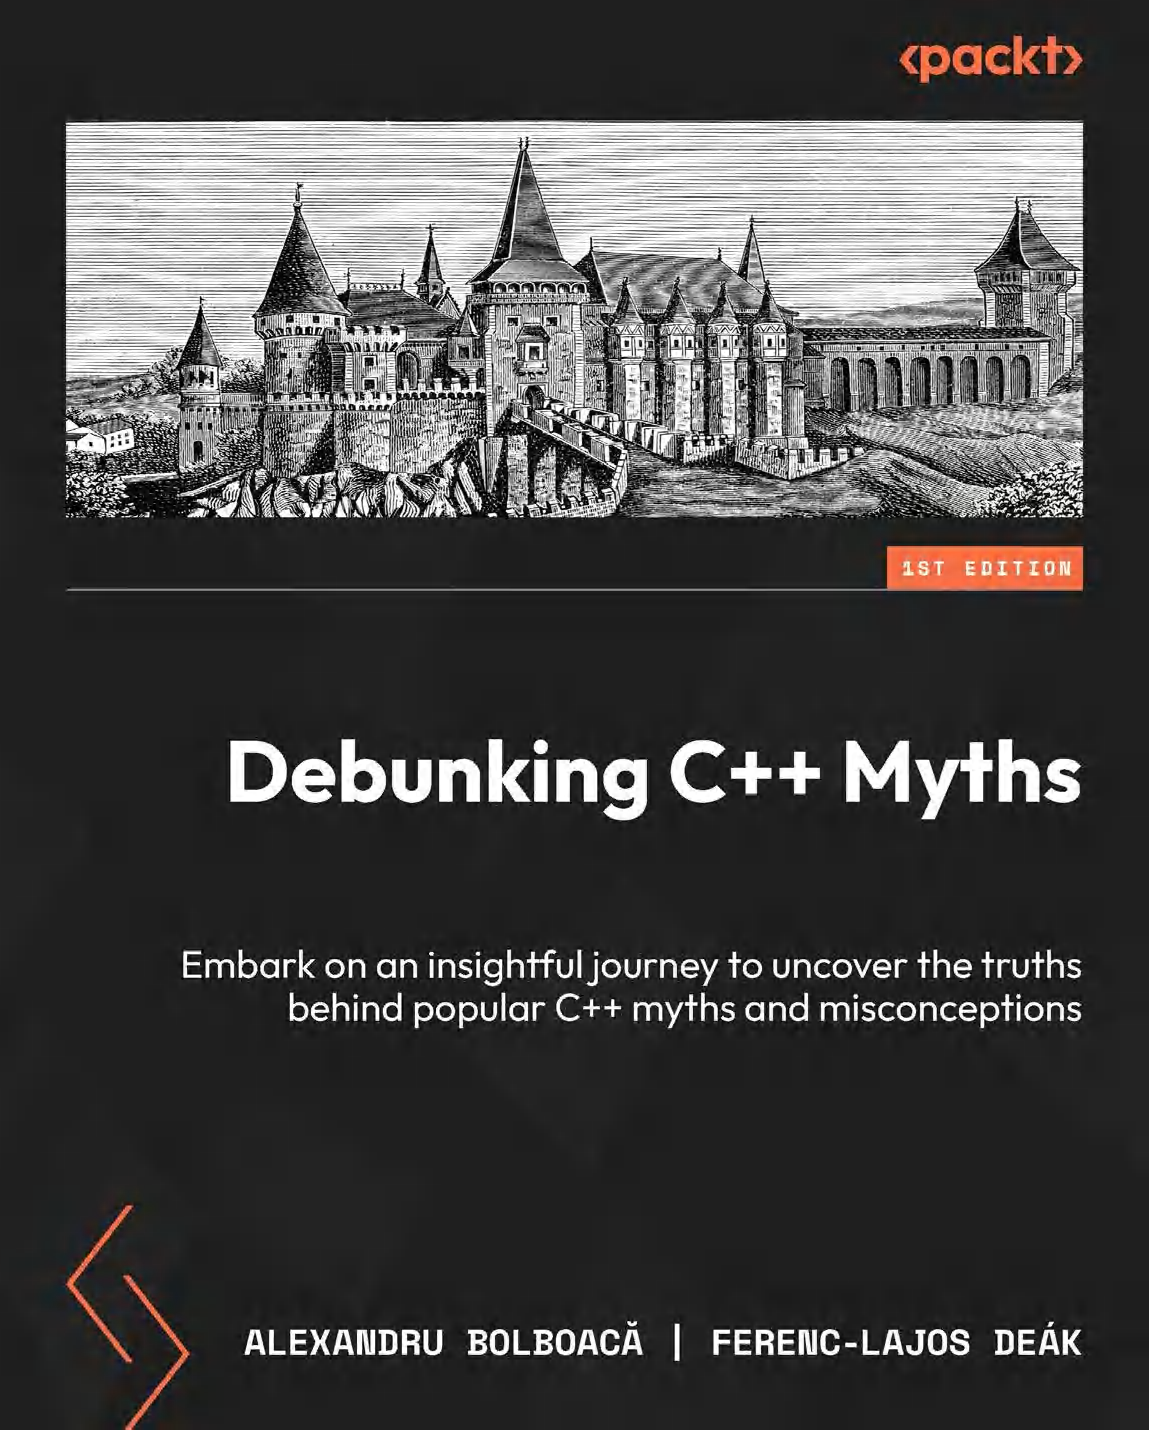
\includegraphics[width=\textwidth,height=\textheight,keepaspectratio]{cover.png}
\begin{tikzpicture}[remember picture, overlay, inner sep=0pt]
\node at (current page.center)
{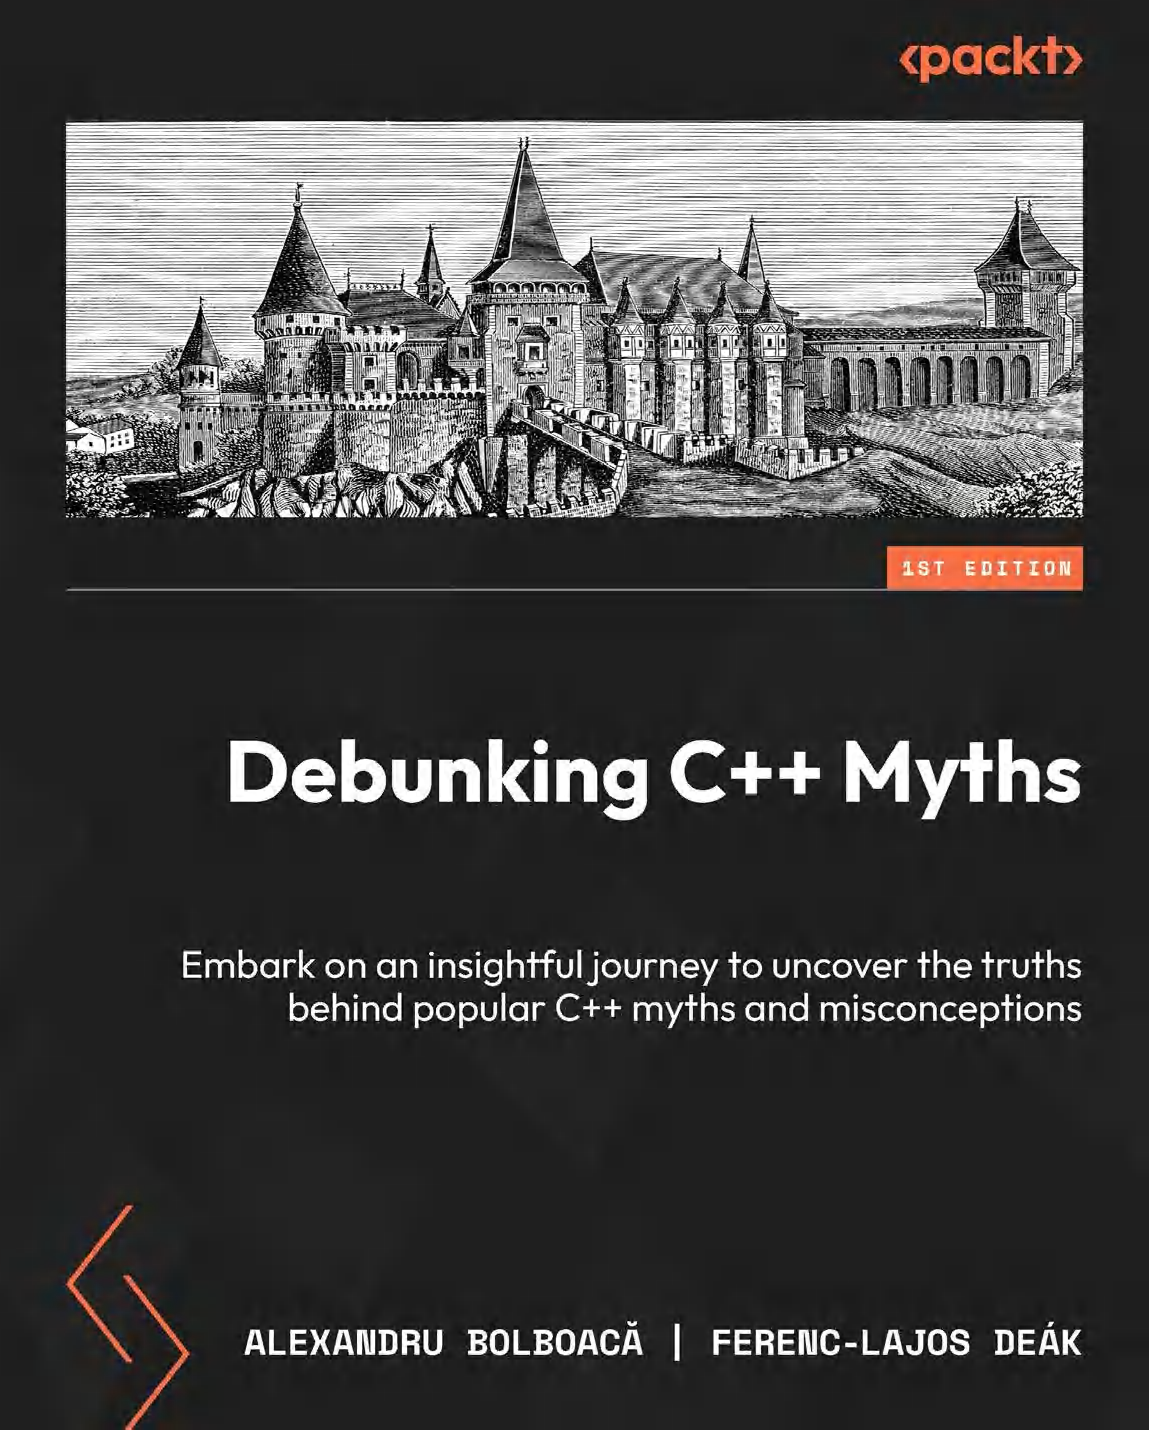
\includegraphics[width=\paperwidth, keepaspectratio=false]{cover.png}};
\end{tikzpicture}
\newpage
\thispagestyle{empty}
\huge
\textbf{走出C++谜云}
\\[9pt]
\normalsize
揭开C++的真相与误解
\\[9pt]
\normalsize
作者: Alexandru Bolboacă, Ferenc-Lajos Deák
\\[8pt]
\normalsize
译者:\href{https://github.com/xiaoweiChen/Debunking-Cpp-Myths}{陈晓伟}
\\[8pt]
\end{center}

\newpage

\begin{comment}
\end{comment}

\pagestyle{empty}
\tableofcontents
\newpage

\setsecnumdepth{section}

\myChapter{致谢}{}{content/dedicated.tex}
\newpage

\myChapter{关于作者}{}{content/about-the-author.tex}
\newpage

\myChapter{关于评审}{}{content/about-the-reviewer.tex}
\newpage

\myChapter{前言}{}{content/preface.tex}
\newpage

\myChapter{第1章}{C++的学习困境}{content/chapter1/0.tex}
\mySubsection{1.1.}{环境要求}{content/chapter1/1.tex}
\mySubsection{1.2.}{为什么难学}{content/chapter1/2.tex}
\mySubsection{1.3.}{C++ 的难点}{content/chapter1/3.tex}
\mySubsection{1.4.}{Stroustrup学习法}{content/chapter1/4.tex}
\mySubsection{1.5.}{Kate Gregory --- 不要教授C语言}{content/chapter1/5.tex}
\mySubsection{1.6.}{测试驱动学习法}{content/chapter1/6.tex}
\mySubsection{1.7.}{能力越大,责任越大}{content/chapter1/7.tex}
\mySubsection{1.8.}{总结}{content/chapter1/8.tex}
\newpage

\myChapter{第2章}{理想与现实:C++程序的边界}{content/chapter2/0.tex}
\mySubsection{2.1.}{环境要求}{content/chapter2/1.tex}
\mySubsection{2.2.}{遥远的加纳某地}{content/chapter2/2.tex}
\mySubsection{2.3.}{微软的 C++}{content/chapter2/3.tex}
\mySubsection{2.4.}{自由编译器}{content/chapter2/4.tex}
\mySubsection{2.5.}{仅为头文件时}{content/chapter2/5.tex}
\mySubsection{2.6.}{鲜为人知的那些事}{content/chapter2/6.tex}
\mySubsection{2.7.}{未来之路}{content/chapter2/7.tex}
\mySubsection{2.8.}{总结}{content/chapter2/8.tex}
\newpage

\myChapter{第3章}{范式之争:C++的多面性}{content/chapter3/0.tex}
\mySubsection{3.1.}{环境要求}{content/chapter3/1.tex}
\mySubsection{3.2.}{多面性}{content/chapter3/2.tex}
\mySubsection{3.3.}{函数式编程}{content/chapter3/3.tex}
\mySubsection{3.4.}{元编程}{content/chapter3/4.tex}
\mySubsection{3.5.}{强类型的极限}{content/chapter3/5.tex}
\mySubsection{3.6.}{忽略类型}{content/chapter3/6.tex}
\mySubsection{3.7.}{总结}{content/chapter3/7.tex}
\newpage

\myChapter{第4章}{程序入口:表象之下的复杂性}{content/chapter4/0.tex}
\mySubsection{4.1.}{main()函数}{content/chapter4/1.tex}
\mySubsection{4.2.}{企鹅(Linux)农场}{content/chapter4/2.tex}
\mySubsection{4.3.}{打开窗户}{content/chapter4/3.tex}
\mySubsection{4.4.}{总结}{content/chapter4/4.tex}
\newpage

\myChapter{第5章}{C++类内秩序的美学}{content/chapter5/0.tex}
\mySubsection{5.1.}{大小很重要}{content/chapter5/1.tex}
\mySubsection{5.2.}{尊重顺序}{content/chapter5/2.tex}
\mySubsection{5.3.}{思考顺序}{content/chapter5/3.tex}
\mySubsection{5.4.}{黑暗法则}{content/chapter5/4.tex}
\mySubsection{5.5.}{顺序不重要时}{content/chapter5/5.tex}
\mySubsection{5.6.}{总结}{content/chapter5/6.tex}
\newpage

\myChapter{第6章}{内存安全的挑战}{content/chapter6/0.tex}
\mySubsection{6.1.}{环境要求}{content/chapter6/1.tex}
\mySubsection{6.2.}{内存安全很重要}{content/chapter6/2.tex}
\mySubsection{6.3.}{旧C++的内存安全问题}{content/chapter6/3.tex}
\mySubsection{6.4.}{现代C++的救赎}{content/chapter6/4.tex}
\mySubsection{6.5.}{现代C++的局限性}{content/chapter6/5.tex}
\mySubsection{6.6.}{仍需努力}{content/chapter6/6.tex}
\mySubsection{6.7.}{总结}{content/chapter6/7.tex}
\newpage

\myChapter{第7章}{并发的艺术与实践}{content/chapter7/0.tex}
\mySubsection{7.1.}{环境要求}{content/chapter7/1.tex}
\mySubsection{7.2.}{并行性和并发性的定义}{content/chapter7/2.tex}
\mySubsection{7.3.}{并行性和并发性的常见问题}{content/chapter7/3.tex}
\mySubsection{7.4.}{函数式编程的救援}{content/chapter7/4.tex}
\mySubsection{7.5.}{Actor模型}{content/chapter7/5.tex}
\mySubsection{7.6.}{我们的能力边界}{content/chapter7/6.tex}
\mySubsection{7.7.}{总结}{content/chapter7/7.tex}
\newpage

\myChapter{第8章}{极致性能:内联汇编}{content/chapter8/0.tex}
\mySubsection{8.1.}{像素觉醒}{content/chapter8/1.tex}
\mySubsection{8.2.}{数字宇宙之和}{content/chapter8/2.tex}
\mySubsection{8.3.}{单指令霸权}{content/chapter8/3.tex}
\mySubsection{8.4.}{总结}{content/chapter8/4.tex}
\newpage

\myChapter{第9章}{C++的另类美学}{content/chapter9/0.tex}
\mySubsection{9.1.}{追求美}{content/chapter9/1.tex}
\mySubsection{9.2.}{零的定义}{content/chapter9/2.tex}
\mySubsection{9.3.}{关于括号}{content/chapter9/3.tex}
\mySubsection{9.4.}{趣谈}{content/chapter9/4.tex}
\mySubsection{9.5.}{总结}{content/chapter9/5.tex}
\newpage

\myChapter{第10章}{缺乏现代库生态的困境}{content/chapter10/0.tex}
\mySubsection{10.1.}{何以见得?}{content/chapter10/1.tex}
\mySubsection{10.2.}{现代开发者的真知}{content/chapter10/2.tex}
\mySubsection{10.3.}{共同的需要}{content/chapter10/3.tex}
\mySubsection{10.4.}{兼容性}{content/chapter10/4.tex}
\mySubsection{10.5.}{供应链安全}{content/chapter10/5.tex}
\mySubsection{10.6.}{总结}{content/chapter10/6.tex}
\newpage

\myChapter{第11章}{兼容性的双刃}{content/chapter11/0.tex}
\mySubsection{11.1.}{C与C++的兼容方向}{content/chapter11/1.tex}
\mySubsection{11.2.}{空格:从必须到无视}{content/chapter11/2.tex}
\mySubsection{11.3.}{auto的惊喜}{content/chapter11/3.tex}
\mySubsection{11.4.}{总结}{content/chapter11/4.tex}
\newpage

\myChapter{第12章}{Rust将取代C++}{content/chapter12/0.tex}
\mySubsection{12.1.}{环境要求}{content/chapter12/1.tex}
\mySubsection{12.2.}{为什么要竞争?}{content/chapter12/2.tex}
\mySubsection{12.3.}{Rust的特性}{content/chapter12/3.tex}
\mySubsection{12.4.}{Rust的优势}{content/chapter12/4.tex}
\mySubsection{12.5.}{C++哪些方面更优秀}{content/chapter12/5.tex}
\mySubsection{12.6.}{为什么仍然需要C++}{content/chapter12/6.tex}
\mySubsection{12.7.}{总结}{content/chapter12/7.tex}
\newpage

\begin{comment}
\end{comment}
